
%%%%%%%%%%%%%%%%% Introduction to the Assignment %%%

In this Assignment, \textit{\textbf{Problem 2 - Problems Optics}}, ...


%%%%%%%%%%%%%%%%% TASK 1 %%%
\section{Working principle of CCD's}
Charged Coupled Devices, in short CCD's, are highly sensitive devices for photon detection, mainly used in digital image sensors. A CCD usually consists of a great number of small units, also called pixels, where the main component is a so-called charge storage capacitor, similar to a p-doped metal oxide semiconductor (MOS) (see Fig. \ref{fig:mos}).
In a common MOS device the charge distribution in the semiconductor is modified, when a voltage is applied across  (from gate to substrate), which is caused by the majority carriers being repelled from the Si-SiO2 junction and thus forming a depletion layer, as can be seen in Fig. \ref{fig:mos} \citep[c.f.][chap. 6.8.1]{hoymorksensors}.

\begin{figure}[!htbp]
	\centering
	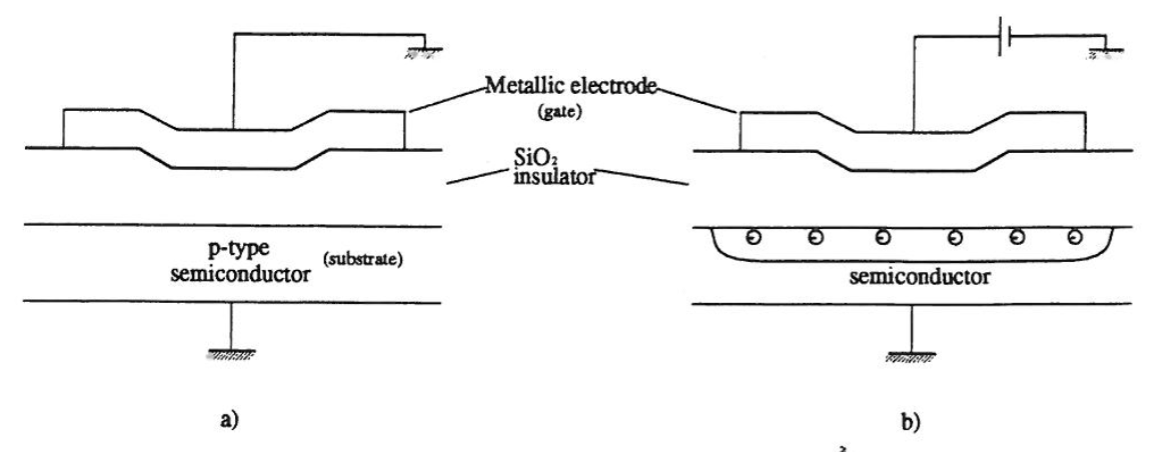
\includegraphics[width=\linewidth]{images/mos}
		\caption{(a) basic MOS capacitor. (b) Depletion Layer under reverse bias \citep[c.f.][fig. 6.20]{hoymorksensors} }
		 \label{fig:mos}
\end{figure}

%If the gate voltage is high enough, an inversion layer forms between the oxide and the depletion layer, which allows 
Due to the photo-electric effect, incoming photons can now generate electron-hole pairs, where the electron is drawn to the positive charged zone and the hole vice versa to the negative charged zone. Therefore, each photon removes a charge from the MOS capacitor, and using a connected charge amplifier, the remaining charge can be converted to a voltage and read out.

 Still, the problem remaining is how to read out individual pixels or MOS capacitors, when there's a large number of them arranged as an array, since connecting every pixel to its individual output amplifier is not suitable or efficient. To cope with this different techniques are used. \par
 According to Hoymark there are four major architectures used for CCD imaging \citep{hoymorksensors}. However, all of them are relying on the same basic principle of charge coupling, which means that the charges accumulated in each pixel are transferred to a charge amplifier by applying appropriate voltages in a time synchronized manner to move charged within the whole CCD device.
 
 The most common techniques are linear shift registers, full frame, frame transfer and the so-called interline transfer.
 For the linear shift register, the simplest of the aforementioned techniques, the CCD is read out horizontally line by line, while the imager or shutter is moving vertically and "scanning" the scene as such.
 The full frame technique uses a global shutter, means the whole CCD is illuminated and read out completely after an appropriate integration time. 
 The third technique, frame transfer is usually used when high frame rates are demanded. Here, only half of the CCD array is illuminated for a specific integration/exposure time and after transferred to the other half where the charges are read out, while the next frame is already captured by the illuminated half.
 However, a disadvantage of the frame transfer technique is "smearing", which means that parts of the captured image are blurry due to the nature of the frame capture.
 Using the interline transfer technique gets rid of this problem by using the CCD 2D array as array of 1D CCD Line sensors. These lines are then connected to an output register which are filled after the line sensors have been illuminated. After, these output register are read out while the next image is already integrated \citep{hoymorksensors}.
 
 Furthermore, the charge coupling can be done using different approaches, more specifically two- three- or four phase cycles which affects the clocking complexity as well as the total amount of gates needed amongst other things \citep{ccdimaging}.
 



%%%%%%%%%%%%%%%%% TASK 2 %%%
\section{CCD Parameters}

\subsection{spectral radiant incidence}

\subsection{number of incident photons}

\subsection{quantum efficiency}
Quantum Efficiency (QE) describes the ratio between the photons hitting the CCD and the photons that are actually detected or collected \citep{hoymorksensors}. The Quantum Efficiency can vary throughout the band-pass\footnote{total spectral range for which a detector is sensitive}, thus having different efficiencies for different colors. Modern CCD's have a band-pass of about 3000 to 10000 Å\footnote{1 {Ångström} equals $10^{-10}$ m} and can reach a QE of up to 90\%, while having a QE of 60\% and more for over two thirds of the spectrum \citep{howellCCD}.

%https://www.noao.edu/meetings/gdw/files/Howell_CCDs.pdf

\subsection{Pixel}
A pixel in a CCD device refers to one single unit of a MOS capacitor device, that is able to convert incoming photons to a respective charge, which then can be converted to an appropriate "brightness level" using an charge amplifier and an appropriate ADC as well as specialised software.

\subsection{Noise and its sources}
\label{chap:noise}
According to Hoymork there are three noise sources that have to be considered: read noise, signal shot noise and pixel-to-pixel pattern noise, or, speaking in astronomy terms "read noise limited", "photon noise limited", and "flat field uncertainties" \citep{howellCCD,hoymorksensors}.
At high signal levels the most noise occurs due to pixel-to-pixel sensitivity, which corresponds to the fixed pattern noise in figure \ref{fig:noise}, whereas during low signal levels the limiting noise is the so-called read noise floor, a noise present because of the device properties \citep{hoymorksensors}.

\begin{figure}[!htbp]
	\centering
	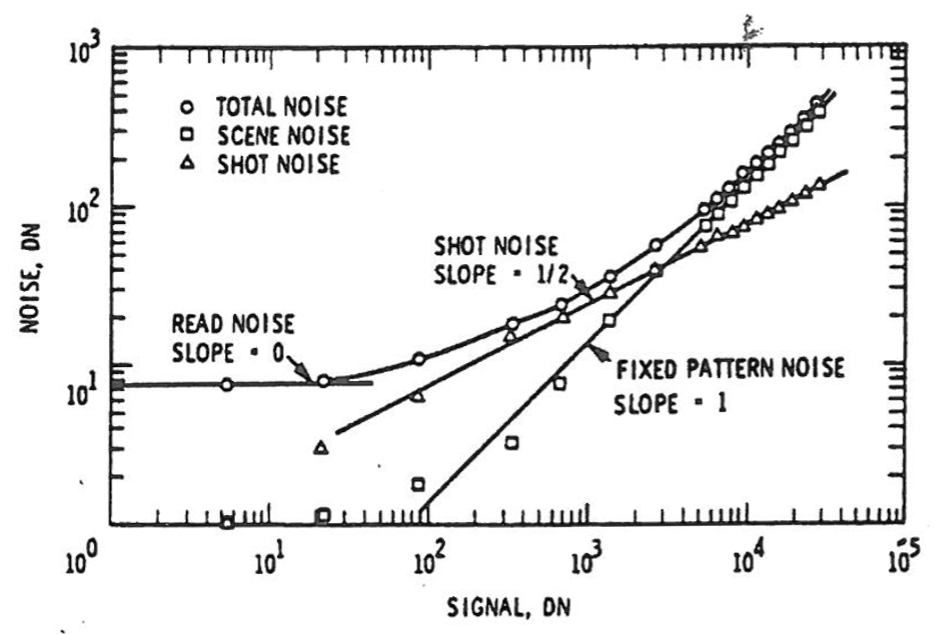
\includegraphics[width=\linewidth]{images/noise}
		\caption{Noise plotted as function of an 20x20 input array \citep[c.f.][fig. 6.24]{hoymorksensors} }
		 \label{fig:noise}
\end{figure}

\subsection{Signal-to-noise ratio for CCD and image intensifier (ICCD)}
In general, the signal-to-noise ratio, in short SNR, characterizes the quality of a measurement. In the case of a CCD the SNR describes the ratio of the total received signal and the combined noise, consisting of the components addressed in chap. \ref{chap:noise} \citep{noiseFSU}. \par
An Intensified CCD (ICCD), is a CCD with an intensifier image tube put in front of the CCD to enhance the sensitivity of the CCD sensor. Applying an intensifier tube reduces the Quantum Efficiency drastically though, which must be considered during design of an instrument or application \citep{hoymorksensors}.

\subsection{Noise- and Saturation Equivalent Exposure}
The Noise Equivalent Exposure is defined as a SNR of 1, which means that signal after exposing/integrating has the same strength as the combined system noise, rendering the measurement more or less unusable. According to Brändström the Detection Threshold is located at an SNR of around 2 \citep[c.f.][chap. 3.1.10]{brandstrom2003auroral}.

The Saturation Equivalent Exposure is the exposure/integration after which the well capacity of the single MOS capacitors of the CCD is fully exhausted. This leads to saturation, as the name implies. Further illumination or more exposure can not be detected \citep{brandstrom2003auroral}.

\subsection{Dynamic Range}
The Dynamic Range (DR) of a sensor is given in dB and is the peak signal divided by the Root-Mean-Square noise and the DC bias level.

In other words, it is the peak signal, which means the maximum achievable signal defined by the well capacity, divided by the sum of noises of the system. For practical applications this means that the higher the dynamic range is, the better low intensity signals are being detected.


\begin{figure}[!htbp]
	\centering
	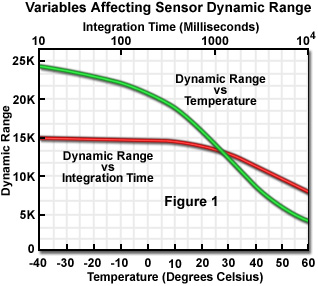
\includegraphics[width=0.6\linewidth]{images/dynrange}
		\caption{Dynamic Range and its Variables\protect\footnotemark}
		 \label{fig:dynrange}
\end{figure}
\footnotetext{source: \url{https://micro.magnet.fsu.edu/primer/digitalimaging/concepts/images/dynamicrangefigure1.jpg}}







%%%%%%%%%%%%%%%%% TASK 3 %%%
\section{CCD Elements for ALIS}
ALIS is an Auroral Large Imaging System proposed by Åke Steen in 1989 to automate auroral imaging stations in Scandinavia. The following chapters describe different elements of the CCD chosen for this specific project \citep{brandstrom2003auroral}.

\subsection{optical system}
The optical system of ALIS 

\subsection{interference filters}

\subsection{camera positioning system}


%%%%%%%%%%%%%%%%% TASK 4 %%%
\section{Scientific results of ALIS}


\subsection{estimation of auroral electron spectra;}

\subsection{auroral vorticity}

\subsection{ionospheric trough}

\subsection{daytime auroral imaging}

\subsection{auroral events and thermospheric neutral wind}

\subsection{meteor studies}



%%%%%%%%%%%%%%%%% TASK 4 %%%
\section{CCD comparison of ALIS and onboard Earth auroral imaging}


%%%%%%%%%%%%%%%%% TASK 5 BONUS %%%
\section{Literature Survey}




